\section{邻近方法}
\label{sec:ns-proximal}

次梯度法慢，一个原因是它在尖点上只用了一个斜率，把“这里是尖的”这个信息丢了。这就需要回答：如果愿意在每一步多做一点计算，怎样把尖点的结构保留在更新里？办法是把一步更新本身写成一个小优化问题。

\subsection{邻近映射}
\label{sec:ns-prox-map}

梯度步有一个等价的写法：对光滑的$f$，$\bm{x}-\alpha\nabla f(\bm{x})$是下面二次函数的最小点，
\[
 f(\bm{x})+\langle\nabla f(\bm{x}),\bm{y}-\bm{x}\rangle+\frac{1}{2\alpha}\lVert\bm{y}-\bm{x}\rVert_2^2.
\]
这里$f$被它的一阶近似代替，再加一个二次距离项，防止走太远。如果$f$的结构足够简单，就不必做一阶近似，直接把$f$本身留在问题里。

\begin{definition}[邻近映射]
\label{def:ns-prox}
设$f:\mathbb{R}^n\to\mathbb{R}\cup\{+\infty\}$是适当、下半连续的凸函数，$\alpha>0$。输入点$\bm{x}$的\term{邻近映射}（proximal mapping）定义为
\begin{equation}
 \operatorname{prox}_{\alpha f}(\bm{x})=\argmin_{\bm{y}\in\mathbb{R}^n}\Bigl\{f(\bm{y})+\frac{1}{2\alpha}\lVert\bm{y}-\bm{x}\rVert_2^2\Bigr\}.
 \label{eq:ns-prox}
\end{equation}
\end{definition}

括号里两项在拉锯：$f$想让$\bm{y}$去函数值低的地方，距离项想让$\bm{y}$留在$\bm{x}$附近，$\alpha$决定谁的话更算数。$\alpha$很小时，结果几乎停在$\bm{x}$；$\alpha$很大时，结果接近$f$的最小点。

图~\ref{fig:ns-prox-geometry}对$f(y)=\lvert y\rvert$，$\alpha=1$画出了这种拉锯。输入$x=2$时，和函数的最小点在$p=1$处，函数值的下降抵得过距离的代价。输入$x=0.6$时，绿色曲线的最小点卡在$y=0$的尖点上：再靠近$x$的收益太小，推不动尖点。

\begin{BookInlineFigure}
  \centering
  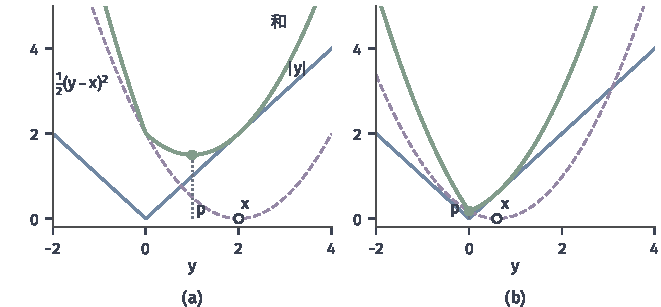
\includegraphics[width=112mm]{figures/05-optimization/03-nonsmooth-optimization/matplotlib/ns-prox-geometry/figure.pdf}
  \caption{邻近映射是一个小优化问题，$f(y)=\lvert y\rvert$，$\alpha=1$。蓝线是$f$，紫色虚线是距离项$\tfrac12(y-x)^2$，绿线是两者之和，绿点是和的最小点$p$，空心圆是输入点。(a)$x=2$，最小点$p=1$位于光滑部分。(b)$x=0.6$，最小点落在尖点$p=0$上。}
  \label{fig:ns-prox-geometry}
\end{BookInlineFigure}

定义中对$f$的要求，下面的定理逐一用到。

\begin{theorem}[邻近映射的存在、唯一与刻画]
\label{thm:ns-prox}
设$f$是适当、下半连续的凸函数，$\alpha>0$。则对每个$\bm{x}$，式~\eqref{eq:ns-prox}有唯一的最小点$\bm{p}$，并且
\begin{equation}
 \bm{p}=\operatorname{prox}_{\alpha f}(\bm{x})\quad\Longleftrightarrow\quad\frac{\bm{x}-\bm{p}}{\alpha}\in\partial f(\bm{p}).
 \label{eq:ns-prox-characterization}
\end{equation}
此外，映射是非扩张的：对任意$\bm{x},\bm{y}$，记$\bm{p}=\operatorname{prox}_{\alpha f}(\bm{x})$，$\bm{q}=\operatorname{prox}_{\alpha f}(\bm{y})$，有
\begin{equation}
 \lVert\bm{p}-\bm{q}\rVert_2^2\leq\langle\bm{p}-\bm{q},\bm{x}-\bm{y}\rangle\leq\lVert\bm{x}-\bm{y}\rVert_2\lVert\bm{p}-\bm{q}\rVert_2.
 \label{eq:ns-firm-nonexpansive}
\end{equation}
\end{theorem}

\begin{proof}
记子问题的目标为
\[
 \phi(\bm{y})=f(\bm{y})+\frac{1}{2\alpha}\lVert\bm{y}-\bm{x}\rVert_2^2.
\]

存在性。适当、下半连续的凸函数有一个仿射下界（上图是闭凸集，用分离定理得到），设$f(\bm{y})\geq a+\langle\bm{b},\bm{y}\rangle$。于是
\[
 \phi(\bm{y})\geq a+\langle\bm{b},\bm{y}\rangle+\frac{1}{2\alpha}\lVert\bm{y}-\bm{x}\rVert_2^2\to+\infty\qquad(\lVert\bm{y}\rVert_2\to\infty).
\]
所以$\phi$的下水平集有界。由第~\ref{chap:optimization}章的结果，下半连续性保证下水平集闭，下水平集紧时最小点存在。

唯一性。$\phi$是凸函数与严格凸的二次项之和，严格凸，严格凸函数至多有一个最小点。

刻画。距离项在全空间有限且可微，和规则取等号，由定理~\ref{thm:ns-fermat}，
\[
 \bm{p}\ \text{是最小点}\quad\Longleftrightarrow\quad\bm{0}\in\partial f(\bm{p})+\frac{\bm{p}-\bm{x}}{\alpha}.
\]
移项即得式~\eqref{eq:ns-prox-characterization}。

非扩张性。由式~\eqref{eq:ns-prox-characterization}，
\[
 \bm{s}=\frac{\bm{x}-\bm{p}}{\alpha}\in\partial f(\bm{p}),\qquad
 \bm{v}=\frac{\bm{y}-\bm{q}}{\alpha}\in\partial f(\bm{q}).
\]
两条支撑不等式
\[
 f(\bm{q})\geq f(\bm{p})+\langle\bm{s},\bm{q}-\bm{p}\rangle,\qquad f(\bm{p})\geq f(\bm{q})+\langle\bm{v},\bm{p}-\bm{q}\rangle
\]
相加，得到次微分的单调性$\langle\bm{s}-\bm{v},\bm{p}-\bm{q}\rangle\geq0$。代入$\bm{s},\bm{v}$的表达式并整理，
\[
 \langle(\bm{x}-\bm{y})-(\bm{p}-\bm{q}),\bm{p}-\bm{q}\rangle\geq0.
\]
这就是式~\eqref{eq:ns-firm-nonexpansive}的左半，右半是Cauchy不等式。
\end{proof}

每个条件都有用处。下半连续保证最小点取得，例如$f$在$(0,1)$内为$0$、其余为$+\infty$时，$\operatorname{dom}f$不闭，$\bm{x}=2$的最小点取不到。凸性保证唯一和式~\eqref{eq:ns-prox-characterization}。若$f=-\lvert y\rvert$，$\alpha=1$，$x=0$，$y=\pm1$都是最小点，映射不再是单值的。

\paragraph{显式步与隐式步}
把式~\eqref{eq:ns-prox-characterization}写成迭代的样子：
\begin{equation}
 \bm{x}^{+}=\bm{x}-\alpha\bm{s},\qquad\bm{s}\in\partial f(\bm{x}^{+}).
 \label{eq:ns-implicit-step}
\end{equation}

形式与次梯度步一样，差别在于斜率取在新点上。显式步先读斜率再走，隐式步要求“走到的地方的斜率正好解释这一步”。由于$\bm{x}^{+}$事先未知，这是一个隐式方程，邻近映射就是它的解。

隐式的好处看两个例子。图~\ref{fig:ns-forward-backward}(a)用$f(x)=\lvert x\rvert$，$x^{(0)}=1$，$\alpha=0.4$。次梯度步的斜率总是$\pm1$，所以点按$0.4$的步子走过零点来回跳，序列是$1,\,0.6,\,0.2,\,-0.2,\,0.2,\ldots$；邻近步在前两步相同，第三步由式~\eqref{eq:ns-implicit-step}选出$s=0.5\in[-1,1]$，恰好落在零上并停住，序列是$1,\,0.6,\,0.2,\,0,\,0,\ldots$。

\begin{BookInlineFigure}
  \centering
  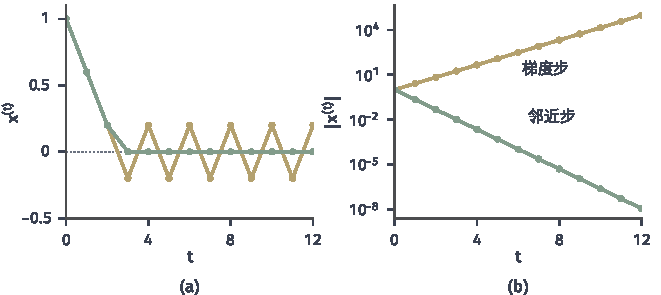
\includegraphics[width=112mm]{figures/05-optimization/03-nonsmooth-optimization/matplotlib/ns-forward-backward/figure.pdf}
  \caption{显式步（黄）与隐式的邻近步（绿）。$\alpha=0.4$，$x^{(0)}=1$。(a)$f(x)=\lvert x\rvert$：次梯度步在零点两侧反复跳动，邻近步第三步后停在零。(b)$f(x)=\tfrac92x^2$：$\alpha$超过$2/L=2/9$，梯度步发散，邻近步对任何$\alpha>0$都收缩，纵轴为对数坐标。}
  \label{fig:ns-forward-backward}
\end{BookInlineFigure}

第二个例子是二次函数$f(x)=\tfrac{c}{2}x^2$，$c=9$。显式与隐式的结果分别是
\[
 x^{+}=(1-\alpha c)x,\qquad x^{+}=\frac{x}{1+\alpha c}.
\]

$\alpha=0.4$时前者的放大倍数$\lvert1-3.6\rvert=2.6$，发散；后者的倍数$1/4.6$，收缩。隐式步对任意$\alpha>0$都不会过冲，见图~\ref{fig:ns-forward-backward}(b)。代价已经写在公式里：$\alpha c$大时要解一个方程，只不过一元时解起来很便宜。表~\ref{tab:ns-explicit-implicit}对比了两者。

\begin{BookInlineTable}
  \centering
  \small
  \begin{tabular}{@{}lll@{}}
    \toprule
     & 显式的梯度或次梯度步 & 隐式的邻近步\\
    \midrule
    更新 & $\bm{x}^{+}=\bm{x}-\alpha\bm{g}(\bm{x})$ & $\bm{x}^{+}=\bm{x}-\alpha\bm{s}$，$\bm{s}\in\partial f(\bm{x}^{+})$\\
    步长限制 & 光滑时$\alpha<2/L$ & 任意$\alpha>0$\\
    尖点 & 跨过去，来回振荡 & 可以停在尖点上\\
    每步代价 & 一次梯度或次梯度 & 解一个带二次项的子问题\\
    是否下降 & 非光滑时不一定 & 总是下降（或已最优）\\
    \bottomrule
  \end{tabular}
  \caption{显式步与隐式的邻近步。两者的数学形式相同，差别在于斜率取在哪个点上。}
  \label{tab:ns-explicit-implicit}
\end{BookInlineTable}

\paragraph{第一个例子：投影}
设$\bm{C}$是非空闭凸集，$f=\iota_{\bm{C}}$。约束指标函数在$\bm{C}$内为零，外面为$+\infty$，邻近子问题变成在$\bm{C}$里找离$\bm{x}$最近的点：
\begin{equation}
 \operatorname{prox}_{\alpha\iota_{\bm{C}}}(\bm{x})=\Pi_{\bm{C}}(\bm{x})=\argmin_{\bm{y}\in\bm{C}}\lVert\bm{y}-\bm{x}\rVert_2.
 \label{eq:ns-projection}
\end{equation}

结果与$\alpha$无关，因为函数值在$\bm{C}$内恒为零。这里$\iota_{\bm{C}}$适当、下半连续、凸的条件，正好要求$\bm{C}$非空、闭、凸。

由式~\eqref{eq:ns-prox-characterization}和式~\eqref{eq:ns-normal-cone}，$\bm{p}=\Pi_{\bm{C}}(\bm{x})$的特征是
\[
 \langle\bm{x}-\bm{p},\bm{y}-\bm{p}\rangle\leq0\qquad\text{对所有}\ \bm{y}\in\bm{C}.
\]
也就是从$\bm{p}$看，$\bm{x}$与$\bm{C}$中任一点的夹角不小于直角。

投影是否好算取决于$\bm{C}$。盒子逐坐标截断，球沿半径缩回。例如$\bm{C}=[-1,1]^2$时，$(2,0.5)$投影到$(1,0.5)$；单位球时，$(3,4)$投影到$(0.6,0.8)$。图~\ref{fig:ns-projection}画出了这两种情形。

\begin{BookInlineFigure}
  \centering
  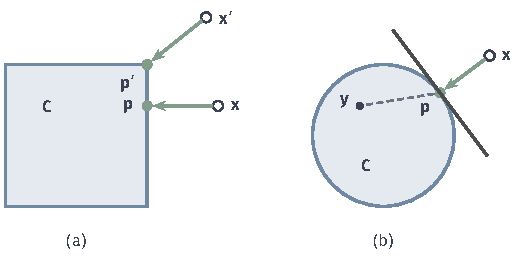
\includegraphics[width=88.4mm]{figures/05-optimization/03-nonsmooth-optimization/tikz/ns-projection/figure.pdf}
  \caption{投影是约束指标函数的邻近映射。浅蓝区域是$\bm{C}$，空心圆是输入点，绿点是投影。(a)盒约束逐坐标截断，$\bm{x}'$落在角上。(b)球约束，深灰线是过$\bm{p}$的切线。集合内任一点$\bm{y}$都在切线的同一侧，从$\bm{p}$看$\bm{x}$与$\bm{y}$夹角不小于直角。}
  \label{fig:ns-projection}
\end{BookInlineFigure}

\paragraph{第二个例子：软阈值}
取$f(y)=\lvert y\rvert$。由式~\eqref{eq:ns-prox-characterization}和式~\eqref{eq:ns-abs-subdiff}，按$p$的符号分三种情形。

若$p>0$，则$(x-p)/\alpha=1$，即$p=x-\alpha$，这要求$x>\alpha$。

若$p<0$，则$(x-p)/\alpha=-1$，即$p=x+\alpha$，这要求$x<-\alpha$。

若$p=0$，则$x/\alpha\in[-1,1]$，即$\lvert x\rvert\leq\alpha$。

三种情形恰好互斥且覆盖全部$x$，合起来得到\term{软阈值}（soft thresholding）算子：
\begin{equation}
 S_\alpha(x)=\operatorname{prox}_{\alpha\lvert\cdot\rvert}(x)=\operatorname{sign}(x)\max\{\lvert x\rvert-\alpha,\,0\}.
 \label{eq:ns-soft-threshold}
\end{equation}

它把靠近零的输入压成零，把其余的朝零移动$\alpha$。向量的$\ell_1$范数按坐标可分，邻近映射就是逐坐标软阈值。阈值由步长乘系数给出，$\alpha\lambda\lVert\cdot\rVert_1$的邻近映射就是逐坐标作用的$S_{\alpha\lambda}$。图~\ref{fig:ns-prox-geometry}的两个输入，由公式得$S_1(2)=1$，$S_1(0.6)=0$，都与图中相符。

图~\ref{fig:ns-prox-maps}(a)是这个映射的图像，粗线的长度$2\alpha$就是原点次微分的长度$2$乘$\alpha$。这条规律具有一般性。(b)是三段折线在$\alpha=1$的邻近映射，用同样的分情形方法，每个分支上$p=x-\alpha a_i$（$a_i$是斜率），两个尖点各对应一段水平线，长度分别是$\alpha$乘$\tfrac32$（$x\in[-1,\tfrac12]$）和$\alpha$乘$\tfrac32$（$x\in[\tfrac52,4]$），正好是$\partial f(0)$和$\partial f(2)$的长度乘$\alpha$。

\begin{BookInlineFigure}
  \centering
  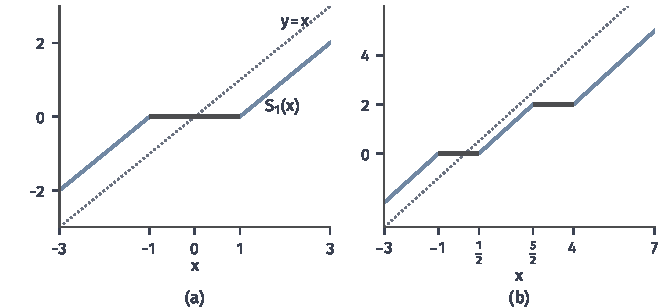
\includegraphics[width=112mm]{figures/05-optimization/03-nonsmooth-optimization/matplotlib/ns-prox-maps/figure.pdf}
  \caption{两个邻近映射的图像（$\alpha=1$），点线是恒等映射。(a)软阈值$S_1$，深灰粗线是被压成零的区间$[-1,1]$。(b)三段折线的邻近映射，深灰粗线是落在尖点$x=0$和$x=2$上的输入区间，长度等于对应次微分的长度乘$\alpha$。}
  \label{fig:ns-prox-maps}
\end{BookInlineFigure}

\subsection{邻近点法}
\label{sec:ns-proximal-point}

既然邻近映射把点往$f$低的方向移，反复应用它会怎样？\term{邻近点法}（proximal point method）就是
\begin{equation}
 \bm{x}^{(t+1)}=\operatorname{prox}_{\alpha^{(t)}f}(\bm{x}^{(t)}),\qquad\alpha^{(t)}>0.
 \label{eq:ns-ppa}
\end{equation}

这是把式~\eqref{eq:ns-implicit-step}反复迭代，每一步的位移除以步长都是新点的一个次梯度。下面的定理说明步长可以任意大，这是显式方法做不到的。

\begin{theorem}[邻近点法的目标差界]
\label{thm:ns-ppa}
设$f$是适当、下半连续的凸函数，存在最小点$\bm{x}^\star$，每一步精确计算式~\eqref{eq:ns-ppa}。则$f(\bm{x}^{(t)})$单调不增，并且
\begin{equation}
 f(\bm{x}^{(T)})-f^\star\leq\frac{\lVert\bm{x}^{(0)}-\bm{x}^\star\rVert_2^2}{2\sum_{t=0}^{T-1}\alpha^{(t)}}.
 \label{eq:ns-ppa-rate}
\end{equation}
\end{theorem}

\begin{proof}
省略上标，把第$t$步的点、新点和步长写成$\bm{x},\bm{x}^{+},\alpha$。由式~\eqref{eq:ns-prox-characterization}，向量$(\bm{x}-\bm{x}^{+})/\alpha$（记为$\bm{s}$）是$f$在$\bm{x}^{+}$的次梯度，所以对任意$\bm{z}$，
\[
 f(\bm{x}^{+})-f(\bm{z})\leq\langle\bm{s},\bm{x}^{+}-\bm{z}\rangle=\frac1\alpha\langle\bm{x}-\bm{x}^{+},\bm{x}^{+}-\bm{z}\rangle.
\]

取$\bm{z}=\bm{x}$，右端是$-\lVert\bm{x}^{+}-\bm{x}\rVert_2^2/\alpha\leq0$，单调性得证。

取$\bm{z}=\bm{x}^\star$，并使用恒等式
\begin{equation}
 2\langle\bm{a}-\bm{b},\bm{b}-\bm{c}\rangle=\lVert\bm{a}-\bm{c}\rVert_2^2-\lVert\bm{b}-\bm{c}\rVert_2^2-\lVert\bm{a}-\bm{b}\rVert_2^2,
 \label{eq:ns-three-point}
\end{equation}
得到
\[
 \alpha\bigl(f(\bm{x}^{+})-f^\star\bigr)\leq\frac12\Bigl(\lVert\bm{x}-\bm{x}^\star\rVert_2^2-\lVert\bm{x}^{+}-\bm{x}^\star\rVert_2^2\Bigr).
\]

对$t=0,\ldots,T-1$相加，距离项相消，右端不超过$\lVert\bm{x}^{(0)}-\bm{x}^\star\rVert_2^2/2$。左端由单调性，每一项的$f(\bm{x}^{(t+1)})\geq f(\bm{x}^{(T)})$，于是
\[
 \Bigl(\sum_{t=0}^{T-1}\alpha^{(t)}\Bigr)\bigl(f(\bm{x}^{(T)})-f^\star\bigr)\leq\frac12\lVert\bm{x}^{(0)}-\bm{x}^\star\rVert_2^2.
\]
两边相除即得。
\end{proof}

分母里是$\alpha^{(t)}$的累积，所以$\alpha$越大收敛越快。一步用很大的$\alpha$，子问题几乎就是原问题，这正是问题所在：式~\eqref{eq:ns-ppa}把难度搬进了子问题，并没有消除它。

用第~\ref{chap:first-order-methods}章的二次目标$f(\bm{x})=\tfrac12(x_1^2+9x_2^2)$，$\bm{x}^{(0)}=(9,1)$演示。对角情形的子问题有闭式解，$\alpha=1$时第一步是
\[
 \bm{x}^{(1)}=\Bigl(\frac{9}{1+1},\ \frac{1}{1+9}\Bigr)=(4.5,\,0.1).
\]

再走一步，
\[
 \bm{x}^{(2)}=(2.25,\,0.01).
\]

图~\ref{fig:ns-ppa-path}(a)中绿色路径没有梯度下降（黄色，$\alpha=1/5$）的折返，(b)说明$\alpha$增大时收敛更快。这个例子每步的工作量几乎为零，但只是因为$\bm{H}$是对角矩阵。一般二次目标的子问题是线性方程组$(\bm{I}+\alpha\bm{H})\bm{x}^{+}=\bm{x}$，$\alpha$越大，它的条件数越接近$\bm{H}$本身，求解代价越接近原问题。

\begin{BookInlineFigure}
  \centering
  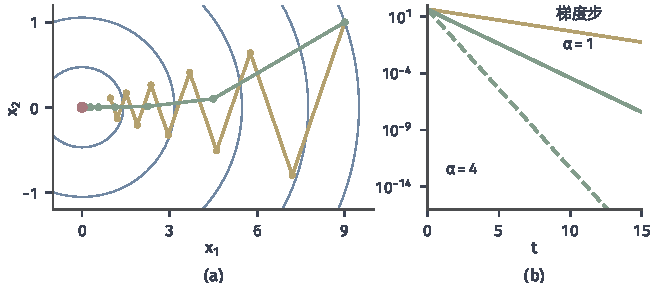
\includegraphics[width=112mm]{figures/05-optimization/03-nonsmooth-optimization/matplotlib/ns-ppa-path/figure.pdf}
  \caption{邻近点法在二次目标$\tfrac12(x_1^2+9x_2^2)$上的表现，$\bm{x}^{(0)}=(9,1)$。(a)等高线（蓝）上的路径，横纵比例不同，绿色为$\alpha=1$的邻近点法，黄色为$\alpha=1/5$的梯度下降。(b)目标差（对数坐标），绿色实线、虚线分别是$\alpha=1,4$的邻近点法，黄色是梯度下降。}
  \label{fig:ns-ppa-path}
\end{BookInlineFigure}

\paragraph{三件事要分别核验}
使用邻近点法时要分清三个问题，它们不能相互代替。

第一，映射可定义。这由定理~\ref{thm:ns-prox}回答，只要$f$适当、下半连续、凸。

第二，子问题可计算。定义合法不等于算得出来。对$\lvert x\rvert$有闭式解，对$\tfrac12(x_1^2+9x_2^2)$有简单公式；对一般的$f$，子问题本身需要迭代求解。

第三，原问题收敛。定理~\ref{thm:ns-ppa}额外要求最小点存在。取$f(x)=e^x$，邻近映射处处有定义，每一步也能用牛顿法算出。$\alpha=1$，$x^{(0)}=0$时，方程$p-x+e^p=0$依次给出
\[
 x^{(1)}\approx-0.567,\qquad x^{(2)}\approx-0.953,\qquad x^{(3)}\approx-1.242.
\]
序列单调趋于$-\infty$，$f(x^{(t)})$趋于下确界$0$，但下确界取不到，也就不存在“收敛到解”这回事。

\paragraph{子问题的精度}
实际中子问题只能算到一定精度。设计算结果与精确的邻近点的距离不超过$\varepsilon^{(t)}$。由非扩张性~\eqref{eq:ns-firm-nonexpansive}，$\bm{x}^\star$是不动点，所以
\begin{equation}
 \lVert\bm{x}^{(t+1)}-\bm{x}^\star\rVert_2\leq\lVert\bm{x}^{(t)}-\bm{x}^\star\rVert_2+\varepsilon^{(t)}.
 \label{eq:ns-inexact-prox}
\end{equation}

只要$\sum_t\varepsilon^{(t)}<\infty$，这个递推就说明序列有界，误差的累积不会把点推走。进一步可证，在$\alpha^{(t)}$有正下界时序列收敛到一个最小点，证明要用到不动点序列的单调性论证，篇幅较长。

若误差不衰减，结果只能到某个精度。用$f(x)=\lvert x\rvert$，$\alpha=0.4$，$x^{(0)}=1$，假设每一步都多偏出$0.1$：
\[
 1\ \to\ 0.7\ \to\ 0.4\ \to\ 0.1\ \to\ 0.1\ \to\cdots
\]
序列停在$0.1$。这里的$0.1$恰好是子问题的误差。把误差取成$\varepsilon^{(t)}=0.1\cdot2^{-t}$后，点最终收敛到零。子问题要算多准，取决于最后想要多准，二者是同一量级的问题，这个经验在后面的邻近梯度法上同样适用。
